% TEMPLATE for Usenix papers, specifically to meet requirements of
%  USENIX '05
% originally a template for producing IEEE-format articles using LaTeX.
%   written by Matthew Ward, CS Department, Worcester Polytechnic Institute.
% adapted by David Beazley for his excellent SWIG paper in Proceedings,
%   Tcl 96
% turned into a smartass generic template by De Clarke, with thanks to
%   both the above pioneers
% use at your own risk.  Complaints to /dev/null.
% make it two column with no page numbering, default is 10 point

% Munged by Fred Douglis <douglis@research.att.com> 10/97 to separate
% the .sty file from the LaTeX source template, so that people can
% more easily include the .sty file into an existing document.  Also
% changed to more closely follow the style guidelines as represented
% by the Word sample file. 

% Note that since 2010, USENIX does not require endnotes. If you want
% foot of page notes, don't include the endnotes package in the 
% usepackage command, below.

% This version uses the latex2e styles, not the very ancient 2.09 stuff.
\documentclass[letterpaper,twocolumn,11pt]{article}
\usepackage{usenix,epsfig,endnotes}
\usepackage{indentfirst}
\usepackage{subfigure}
\usepackage{color}
\usepackage{array}
\usepackage{longtable}
\usepackage{calc}
\usepackage{multirow}
\usepackage{hhline}
\usepackage{ifthen}
\usepackage{url}
\begin{document}

%don't want date printed
\date{}

%make title bold and 14 pt font (Latex default is non-bold, 16 pt)
\title{\Large \bf Preserving Interactivity of GUI Applications}

%for single author (just remove % characters)
\author{
{\rm Hilfi Alkaff}\\
hilfialkaff@berkeley.edu
\and
{\rm Vu Chiem}\\
vuchiemh@berkeley.edu
\and
{\rm Andrew Wang}\\
awang@eecs.berkeley.edu
% copy the following lines to add more authors
% \and
% {\rm Name}\\
%Name Institution
} % end author

\maketitle

% Use the following at camera-ready time to suppress page numbers.
% Comment it out when you first submit the paper for review.
%\thispagestyle{empty}


\subsection*{Abstract}
The manycore machines of the future will likely run a diverse set of concurrent workloads. This places additional demands on resource allocation and scheduling policies of the operating system to ensure interactive behavior of foreground user applications while running high throughput batch processing jobs in the background. In our paper, we show that a degree of performance isolation can be achieved on Linux through the use of the existing cpuset mechanism for realistic GUI applications.

\section{Introduction}

Computer architecture is undergoing a fundamental shift that dictates an equally fundamental shift in operating systems. Moore's law is now being applied to CPU cores rather than clock rate, meaning that commodity processors could soon be have tens, even hundreds of cores. Current operating systems are not well suited for this ``manycore'' future; recent research indicates that scaling of the base operating system itself might not be an issue~\cite{linux:osdi10}, but still leaves open the problem of how to gracefully run a variety of concurrent applications with different performance and resource requirements, especially on single user systems.

Already, running a parallel kernel build while watching a movie degrades framerates to unwatchable levels~\cite{DBLP:conf/osdi/YangLBKM08}. This will only be exacerbated by manycore architectures, since users are likely to simultaneously run a mix of highly parallel interactive, real-time, and batch jobs~\cite{liu09tessellation}. This puts additional stress on schedulers, requiring that they present the right tradeoff between latency-sensitive, real-time, and throughput applications without putting too much additional burden on users or application programmers to manually specify policies. These requirements are already found in specialized applications such as state-of-the-art humanoid robotics, which have very demanding hard and soft real-time requirements~\cite{Yoo:2009:RPD:1618617.1618723, Kaneko04humanoidrobot}. 

It is clear that the current generation of best effort schedulers do not meet these demands. Moreover, this variety of scheduling requirements also applies to resources other than CPU time, such as disk and memory I/O, network access, and CPU caches. For an application to provide high-level performance guarantees to the user, operating systems must provide holistic guarantees to applications regarding all types of system resources.

This can be phrased as applications requiring \textit{performance isolation} even under contention for shared resources. This problem is addressed by the Tessellation research operating system through two mechanisms: space-time partitioning and two-level scheduling~\cite{liu09tessellation}~\cite{tessellation-hotpar10}. These mechanisms are achieved through novel software/hardware integration, one key aspect being microkernel-style services that each implement a single OS function, and can provide their own service level agreements based on their resource allocation. Further detail is deferred to the Tessellation references, but these mechanisms allow Tessellation to make strong space-time resource guarantees such as ``2 cores for 50\% of the time'' or ``500 disk I/O operations a second'' to applications. Given these guarantees, applications can then make their own assurances about their performance to the user, attaining performance isolation.

Our contribution is taking some of these ideas from Tessellation and translating them to a recent Linux distribution. We started with the goal of decomposing a number of GUI applications into services that each provide a specific, limited function, and then using Linux's CPU pinning mechanisms to assign each service its own core. Our work resulted in a modified, service-oriented version of the Qt GUI application framework as well as a resource allocation daemon that can provide strong resource guarantees to our Qt GUI applications. We compare two realistic Qt applications under idle and loaded conditions to show that this approach does not impose a significant performance overhead and that it performs far better in terms of throughput and interactivity under resource contention.

One longer-term goal that influenced our project is porting Qt to Tessellation OS. Ideally, this system would have been built on top of Tessellation to begin with, but due to the pre-alpha stage of the Tessellation code base, required functionality for a Qt port (such as a graphics driver, shared memory, and interprocess communication) were not in a state ready to support our project. However, many of our design and implementation decisions were still heavily influenced by this long term porting goal. Some aspects of our system assume the existence of proposed Tessellation OS functionality (such as lightweight user-level interrupts), making our system relatively less efficient than a traditional Linux version.

\section{Related Work}

Redline~\cite{DBLP:conf/osdi/YangLBKM08} provides a way to ensure responsiveness for real-time and interactive GUI applications via specifications. Specifications describe the application resource requirements such as CPU time slices, memory, and I/O priority. The administrator or user would provide a single, static specification for each application manually, and the resource managers would take into account these requirements when the application is scheduled to run. Our work is very similar to Redline, except that we provide an explicit resource allocation daemon (RS), to which the applications can request for resources dynamically at run time, possibly with different requirements in each request.

Our work shares a common goal with AIRS~\cite{kato:airs:} in that they both strive to maintain interactiveness of applications even under heavy loads. AIRS takes into account the dynamic resource requirements of applications under loads, as opposed to static specifications in Redline, and it exports a set of APIs with which the applications can express the resource constraints and requirements. This is closer to our concept of the resource allocation daemon; the difference is that AIRS is a scheduler and our mechanism is a user-space traditional Unix daemon.

There exist the operating systems such as fos~\cite{Wentzlaff:2009:FOS:1531793.1531805}, Corey~\cite{Boyd-Wickizer:2008:COS:1855741.1855745}, and Barrelfish~\cite{Schüpbach08embracingdiversity} that are designed for scalability on many-core machines. They complement Tessellation in moving away from shared-memory programming model and locking to message-passing communication style. By removing the needs for locking and therefore cache coherence overhead, the applications can be more scalable. This idea directly influences our design of channels, which is a lock-free, message-passing communication mechanism.

Ideas from Tessellation's two-level scheduling can describe our RS daemon and Lithe~\cite{Pan:2010:CPS:1809028.1806639}~\cite{Pan:2010:CPS:1806596.1806639}. RS daemon provides the first-level scheduling, which is to allocate the necessary hardware resources to applications, while Lithe does intra-process scheduling to let the applications cooperatively manage their allocated resources. Lithe's argument is that only the applications know the best context-switching points and will cooperatively yield resources; this helps to remove inter-process cache interference and other performance-degrading problems. Together, our RS daemon and Lithe can be combined to manage hardware resources at the systems level and let the applications figure out the efficient scheduling at the same time. This is consistent with the evidence presented in Exokernel~\cite{Engler:1995:EOS:224056.224076}~\cite{Engler:1995:EOS:224057.224076}, which shows that the applications can benefit greatly given explicit control over machine resources.

\section{Implementation}

\begin{figure*}[ht]
  \begin{center}
    \subfigure[Monolithic stack]{\label{fig:stack}\includegraphics[scale=0.35]{stack.ps}}
    \subfigure[Service-based approach]{\label{fig:services}\includegraphics[scale=0.35]{services.ps}} \\
  \end{center}
  \caption{Comparison of default and channels-based Qt implementations}
  \label{fig:implementation}
\end{figure*}

A comparison between the current, monolithic Linux GUI application stack and our service-oriented approach is shown in Figure \ref{fig:implementation}. We have removed a significant amount of code from the picture by running directly on a framebuffer, removing the need for a complicated graphics driver, X server, or window manager. These responsibilities are instead split between the I/O service and the applications in our model and are comparatively much less code. This makes it easier to make guarantees about the responsiveness of different parts of the system, and will simplify our porting effort to Tessellation.

The first application to run in our system is the resource allocation daemon (RS), which must manage allocation for the rest of the components in the system. The nameserver (NS) is the second service to start up, which enables service discovery by clients and other services. Ideally, both of these services would be part of the system boot process; such as will be the case in Tessellation.

The I/O service, upon startup, registers itself with the nameservice under a well-known name. Applications can then connect to the I/O service by asking the nameserver for a new communication channel to the I/O service's well-known name. Following that, the I/O service and application use this new channel to share initialization information and setup state. User mouse and keyboard events are all sent to the I/O service, which forwards them to the correct application.

%In this section, we will tie each of the components of the system described earlier to provide a holistic view on the chronology of events. At the beginning, it will only be resource allocation daemon who is running. Then, the nameserver will come along and requests its share of the CPUs to the daemon. The necessary services (in the scope of our paper, only I/O service) and the client applications will do the same too. 
%
%After that, the I/O service will try to register itself to the nameserver. If the nameserver permits the registration, the service will be saved in the nameserver's database for future lookups. Failure of registration will result in termination of the service immediately because that can only mean an alien service is trying to be registered or that the nameserver is too busy to accept another service. Following that, whenever a client application starts and request communication with the I/O service, the nameserver will look for the name of the service. If the service is found in its database, the nameserver then hands a unique id of the channel that is going to be used for the communication between the client and the service and the pid of the service that is to be used for the signalling mechanism. The nameserver is going to reject the client if the service does not have any free channel id though.
%
%When that step is completed, the client just needs to do a simple handshaking protocol with the service, letting it know that there's a client that wants to talk to it. The client could then freely discuss with the service to be guaranteed its share of the resources that the service is holding.

\subsection{Channels}

One of the core elements of Tessellation OS is a form of message passing-style interprocess communication called channels.
Channels are lightweight, asynchronous, lock-free, and only support communication between two processes. This is advantageous over traditional forms of IPC (such as shared memory or sockets) since channels are well-defined points of communication that provide performance and security isolation between processes~\cite{tessellation-hotpar10}.

Our channel implementation depends upon non-blocking buffers, described by Kim, Colmenares, and Rim~\cite{Kim:2007:EAN:1260991.1261857}. A non-blocking buffer is essentially a circular buffer in shared memory that supports a single producer and single consumer. Instead of using a lock, it relies on the atomicity of integer reads and writes along with multiple integer counters to synchronize access. Our channel implementation uses two of these unidirectional buffers to form a single, bidirectional channel.

One design choice we made was the notification mechanism to inform another process that there is new data available in the channel. There are two basic approaches here: asynchronous notifications through a Unix signal or other interrupt, or relying on the receiving process to poll when it is ready to handle more data. Our default policy is a combination of the two; the sender uses Unix signals to interrupt the receiving process when it places new data in the buffer. The signal handler of the receiving process is then expected to poll until the buffer is empty. An examination of the tradeoffs between polling and interrupts is left to future work; our default policy represents a balance between ease of use and performance.

Channels also provide a far richer API than non-blocking buffers. The first, and most obvious, is the construction of synchronous read and write calls built on top of the asynchronous versions. We also provide a number of functions that allow processes to specify a custom signal handler, and implement an internal delay buffer to hold items that have already been read from the non-blocking buffer but are not ready to be handled by the application.

All in all, our channel implementation weighs in at a total of 777 SLOC.

\subsection{Nameserver}
The nameserver functions similarly to a DNS server for channel IPC. It allows services to register themselves under an ASCII string {\tt name}, which can then be used in other applications and services. When a subsequent request is placed for this {\tt name}, the nameserver creates a new shared memory region, initializes a new channel in this shared memory, and then sends the shared memory ID to both processes. The service and client go through a short handshaking protocol, and all further communication between the service and client happen without more nameserver intervention.

There is a slight chicken and egg problem here, since an application needs to already have a channel open to the nameserver before it can request channels to be opened. This is handled by reserving a single globally known shared memory ID for an initialization channel. Access to this channel is controlled via the use of a lock. Upon startup, a process will attempt to access this initialization channel, and uses it to inform the nameserver of its presence. The nameserver will then initialize a new channel and inform the new process of its location; all further communication between the nameserver and the process will then happen over this new channel. Since this initialization channel is only used once during the startup of each process, there is little lock contention.

\subsection{Qt Embedded}

The I/O server and GUI applications are all written within the Qt Embedded framework. The primary reason we chose to modify Qt Embedded was because of its advertised ease of porting to other platforms. Qt Embedded already provides support for Embedded Linux, Windows Mobile, Symbian, and MeeGo, and has minimal architecture and OS requirements for further porting efforts to Tessellation OS~\cite{qtembedded}.

Since Qt Embedded is designed for embedded platforms, it runs directly on a framebuffer with its provided software renderer, removing the need for a real graphics driver, the X stack, or a window manager. This greatly simplifies our system diagram (Figure \ref{fig:implementation}) and makes the prospect of porting it to Tessellation much more feasible; this ease of porting has been leveraged by at least one other operating system research project we are aware of~\cite{ibos}. 

Qt Embedded is structured as a service/client model that separates the responsibilities of receiving and handling user interaction, as well as the responsibilities of rendering and drawing to the screen. The I/O service initially receives all mouse and keyboard events and forwards them to the correct client application. The application then processes the event and renders any changes to a shared memory region. The service is then responsible for using the graphics driver to copy the rendered image to the screen. This division of responsibilities made Qt Embedded a natural target for our project.

Keyboard and mouse events are by default passed from the I/O service to the client application over a local TCP socket. This presented a clean interface for substituting in channel-based communication; we ended up implementing Qt's QAbstractSocket API without major changes to the I/O service or client, indicating that this style of socket communication might fit within the point-to-point channel paradigm.

One of our desired, but unimplemented, features was splitting the graphics rendering and drawing to the screen into a separate service. This would have enabled interesting policies, such as having the window manager rendering only the foreground window as a form of load shedding, or presenting a degraded degree of quality. It also would have removed a dependency on Linux's shared memory mechanisms, instead passing rendered images over channel IPC.

The applications we chose for testing were demo applications packaged with the Qt source code. Since all of our modification efforts were in the underlying framework, the applications themselves required no source changes to run on our version of Qt Embedded. This means that porting applications to our system is essentially free; we were successfully able to run a web browser, animation demo, text editor, raytracer, and image viewer. Ultimately, we chose the web browser and text editor for evaluation; we are also seeking to port more complicated Qt applications to our system.

\subsection{Resource Allocation Daemon}

The resource allocation daemon is one of the most crucial parts of the system. It uses Linux's existing {\tt cpuset} mechanism to group tasks into sets, and then pin each set to a subset of CPU cores. This is a strong isolation mechanism; once added to a cpuset, a process will only run on the cores assigned to that cpuset~\cite{cpusets}.

There are a number of similar mechanisms on Linux that can also be used for pinning processes to cores (e.g. {\tt pbind}, {\tt sched\_setaffinity}), but cpusets have a few advantages over the alternatives. Cpusets make management of a large number of processes easier because they can be hierarchically nested (i.e., sets within sets). They are also persistent across, and can be configured to automatically assign new processes to a default set. Cpusets are also exposed through a special {\tt /dev} interface, meaning they can be manipulated directly from the command line without special tools.

The clearest explanation of the functionality of the resource allocation daemon is through example. When the daemon is started up, it creates a default cpuset to which it grants access to all cores on the system. The daemon then moves all running processes to this default cpuset; this has the additional effect of assigning all future processes to this set, because all forked children of processes in the set start in the same set as their parent.

Processes that wish to be isolated have to explicitly query the resource allocation daemon for a new core. The daemon will then examine the number of cores already being used by isolated processes. If there are still cores available, the daemon will create a new cpuset, allocate it exclusive access to an unused CPU, and then move the process to this new cpuset. When an isolated process finishes running, the daemon recovers the core and adds it back to the default cpuset for further use.

\textbf{Limitations.} This initial implementation is admittedly rudimentary; it can only allocate CPUs at the granularity of entire cores, it does not handle other resources such as memory, cache, or the hard drive, and does not have any policy mechanisms whatsoever. These are all limitations tackled by Tessellation's two-level scheduling and space-time partitioning; together, they allow for dynamic, fine-grained policies regarding many types of resource allocation; we defer to their publications for full details~\cite{liu09tessellation}~\cite{tessellation-hotpar10}.

\textbf{Service/client allocation.} There is one more important aspect of resource allocation that we wish to highlight. When applications are heavily dependent on system services, it is desirable for the service to be able to ``bill'' the client for actions taken on its behalf. This can be done in either a bottom up or top down approach. In the former, a service is given an allocation of resources, and decides internally how best to split time among its clients. In the latter, clients are instead given an allocation that they can give out to services to perform actions on their behalf.

The core difference in these two models is where policies are enforced; the bottom up approach complicates services, which need to be able to maximize utility among their client applications, while the top down approach complicates applications, which will need to maximize their utility across multiple services.

\section{Evaluation}

\subsection{Test setup}

\begin{figure*}[t]
  \begin{center}
    \subfigure[Sunspider JS benchmark]{\label{fig:sunspider}\includegraphics[scale=0.75]{sunspider.ps}}
    \subfigure[Textedit latency measurements]{\label{fig:textedit}\includegraphics[scale=0.75]{textedit.ps}} \\
  \end{center}
  \caption{Comparison between unmodified and channels-based versions of Qt}
  \label{fig:benchmarks}
\end{figure*}

The test harness used was a commodity desktop PC with a quad core Intel i7-870 processor clocked at 2.93 GHz with 4GB of RAM. Hyperthreading, Turbo Boost, and power states were all disabled to normalize the performance of the CPU cores. Loaded conditions were simulated by running 128 CPU-bound background threads. This number is somewhat arbitrary, but a lower or higher number of threads would likely result in a proportional change without affecting our conclusions.

We encountered difficulties in getting both the modified and unmodified version of Qt to run correctly on an actual framebuffer. As a substitute, all tests were run on the Qt Embedded virtual framebuffer, an X11 application used for testing. This means there are additional layers of software, such as X11 and the WM, that interpose between user input and the I/O service. However, our timings are done above these layers, and we believe that this favors neither the unmodified nor channels-based version of Qt.

\subsection{Channels}

To show that our channel implementation was not bottlenecking our Qt applications, we wrote a variety of stress test and benchmarking suites to test latency, throughput, and correctness. As shown in Table \ref{tab:channel}, our channel implementation handles sending these types of messages with latency in the range of microseconds with linear increase in throughput as the message size increases (up to 1KB). This indicates that the overhead from the new data signal notification mechanism totally dominates message copying times for small packet sizes.

Profiling of client / service communication revealed that the vast majority of messages being sent between the I/O service and application were small (in the range of 4-24 bytes) with a few that were a bit larger ($<$200 bytes). This unfortunately falls on the lower end of our channel's performance spectrum, but the rate at which keyboard and mouse events is relatively low and limited by user interaction. This means that 2.5MB/s of throughput is still more than sufficient for our purposes. More importantly, messages are sent with near-microsecond latency, which is far faster than can be perceived.

\begin{table}[tp]
\centering
\begin{tabular}{| l | l | l |}
\hline
Msg size	&Rate (MB/s)		& Latency ($\mu$s) \\ \hline
4B		&2.5	& 1.53 \\
32B		&20.1	& 1.52 \\
512B	&280.0	& 1.74 \\
1024B	&583.5	& 1.67 \\
\hline
\end{tabular}
\caption{Channel benchmarks}
\label{tab:channel}
\end{table}

\subsection{Web Browser}

The first user application we chose for testing was a simple Qt web browser based on WebKit, included with the Qt source code. Browsers are one of the most commonly used and installed user applications, making this Qt web browser a representative choice as a ``real world'' application. Testing browser performance is also easy through the use of a wide variety of Javascript benchmark suites, such as SunSpider~\cite{sunspider}, Kraken~\cite{kraken}, and V8~\cite{v8benchmark}.

We chose to use Apple's SunSpider JS benchmark, which is mostly CPU-bound. Figure \ref{fig:sunspider} shows the time to complete SunSpider, lower being better. In the no load case, the unmodified version of Qt performs roughly three times faster than our version. This is somewhat disappointing; our current guess is that signal handling within the channels is triggering enough context switches to trash the CPU cache, but even this seems unlikely to cause a 3x decrease in performance.

However, the tables are turned in the loaded situation. Our version of Qt maintained roughly equivalent performance, while the unmodified version's performance degraded by more than a factor of 20 (and 7 times worse than our version). This is due to the performance isolation guaranteed by cpusets and the resource allocation daemon; Qt-C is guaranteed its allocation of the CPU even under load, while Qt has to share the CPU with other tasks and experiences additional scheduling and context switching overhead.

\subsection{Textedit}

The second application we chose was the rich text editor, also included as one of the demo applications with the Qt source code. Compared to a browser, a text editor is a relatively simple application, but we feel it is a better test of interactive behavior. Users are likely to be less tolerant of jitter and latency in a text editor because of the expectation of immediate feedback on the screen and the near constant interaction through typing. 

To this end, we instrumented both Qt and Qt-C to measure the time it took an event arriving at the I/O service to be received and handled by the client. Keyboard and mouse events representative of normal usage were then fed to the textedit. As illustrated in Figure \ref{fig:textedit} and Table \ref{tab:textedit_table}, Qt-C performs far better than Qt in terms of latency and variance in latency, with unmodified Qt performing highly erratically under load. This aligns with our own anecdotal experiences using both versions under load; with normal Qt, there is a noticeable delay in words appearing on screen, while the effect on the Qt-C version is imperceptible.

\begin{table}[htp]
\centering
\begin{tabular}{|l | l | l | l |}
\hline
	&Latency ($\mu$s)	&Median	&Std dev\\ \hline
Qt, NL	&0.14	&0.13	&0.049\\
Qt, L	&30.60	&16.67	&37.24\\
Qt-C, NL	&0.16	&0.18	&0.033\\
Qt-C, L	&0.26	&0.15	&0.42\\
\hline
\end{tabular}
\caption{Textedit interactivity}
\label{tab:textedit_table}
\end{table}

\subsection{Further concerns}

In this section, we wish to address a number of concerns that either fall outside of scope or remain unanswered by our analysis.

\textbf{Batch processing throughput.} The coarseness of the cpuset mechanism means that the only way to give a strong resource guarantee to a process is to allocate at the level of entire cores. This clearly will have a strong effect on the throughput of background batch processing jobs (simulated in our case by load generating threads), since they are unable to use the cores allocated to GUI related processes. This effect was exacerbated by the low core count of our test machine; of its four cores, three were allocated to the service, client, and resource allocation daemon, leaving just one out of four for all remaining system processes and thus one fourth the throughput in our background jobs. However, this is not nearly as dire as it may seem; better timesharing of resources and increasing core counts will reduce the relative loss in performance.

\textbf{RS with unmodified Qt.} Given that unmodified Qt also has the same service/client model, it is possible to combine it with the resource allocation daemon to get the same resource guarantees. We expect that this combination would actually be more efficient than our pairing, since socket communication is comparatively more efficient than our interrupt heavy channel implementation). However, this is somewhat orthogonal to the ultimate goal of porting to Tessellation. Tessellation provides a number of facilities that will greatly improve efficiency, such as lightweight user level signals, finer grained resource scheduling policies, and more explicit control over communication. We plan on further exploring this tradeoff between background and foreground tasks once the porting effort is complete.

\section{Future Work}

\textbf{Porting.} As stated elsewhere in the paper, porting to Tessellation will have many performance and efficiency benefits. Channel support should be greatly improved due to lightweight user level interrupts and hardware support for message passing style communication. Many of the other components of Tessellation, such as two level scheduling and fine grained resource allocation, will further improve performance and enable more interesting work into scheduling and resource allocation policies.

\textbf{Composable SLAs.} One of the key questions being examined by Tessellation group is whether there is an ``SLA explosion'' effect due to nested service dependencies. These dependencies of services on other services could rapidly degrade performance guarantees, due to the additional uncertainty added with each layer. The question is whether existing operating systems suffer from this type of deep nesting of services, and if so, can operating system services can be structured in such a way to avoid this problem.

\textbf{Policy.} Resource allocation and scheduling policies is one of the more interesting thrusts for further work. Some of are ideas are to implement forms of load shedding in services as a method of graceful degradation, integrating dynamic priorities for applications based on user interaction, and automatic profiling of how resource allocation affects application performance.

\textbf{Decomposition.} Our implementation only touches on the possibilities for decomposition for GUI applications. As mentioned earlier, there are many core system functions that could be made into services for more consistent performance, such as the network driver, disk I/O, and screen drawing. There is also room for further decomposition within an application; it is easy to imagine a complex application such as a web browser being divided into separate parts based on realtime, latency, and resource requirements.

\textbf{Parallelism.} 

One big aspect of performance amelioration is through parallelism. As time passes, there will be more and more cores in a CPU and our system should exploit that. Currently, our nameserver and resource allocation daemon is single threaded and although Qt uses multi-threading for the client applications and the services, we are pretty sure that they are not parallelized thoroughly yet. 

In order to improve the performance further, we should decompose a more complicated client applications to be served by more number of services. Take the browser as an example. The browser could have its html parser as one service and the lexer as one service. Even more, we could distinguish the service that handles html display from the service that handles flash display.

\section{Conclusion}

In this paper, we have presented a proof that the research direction, i.e. cores partitioning, of Tessellation OS is one candidate for the winning solution in the era of many-cores. We have demonstrated a satisfying performance on intricate, real-world applications. Whether we will need a new operating system or not to preserve the interactivity of applications will be another unanswered question in our paper. This might be solved if we are able to successfully port our system to Tessellation and does experiments with it.

\section{Acknowledgements}

The inspiration for this project, and many of the ideas, were drawn from the Par Lab Tessellation OS group, in particular John Kubiatowicz and Juan Colmenares. 

\section{Availability}

All of our code is available under a dual GPL/LGPL open source license at~\url{http://www.github.com/~azuriel/Qt-channels}

\footnotesize{\bibliographystyle{acm}
\bibliography{bibliography}}

%\theendnotes

\end{document}

